\documentclass[10pt]{beamer}

\usepackage[utf8]{inputenc}
\usepackage{pgfpages}
\usepackage{dirtree}
\setbeamertemplate{note page}[plain]
\setbeameroption{show notes on second screen =left}
\AtEndNote{\vfill \begin{center} mm:hh \end{center}}
\newcommand{\notedir}[1] {
  \note{\dirtree{#1}}}
\usepackage{tcolorbox}
\usepackage{tikz}
\usepackage{tikz-3dplot}
\usetikzlibrary{intersections,calc,,angles,quotes,through}
\usepackage{amsmath}
\usepackage{graphicx}
\usepackage{cases}
\def \heart {\textcolor{blue}{$\heartsuit$} }
\def \C {\mathcal{C}}
\def \orthog {\underline{\perp}}
\def\arcos{\operatorname{arcos}}
\def \deg {^{\circ}}

\newcommand{\vect}[1] {
  \overrightarrow{#1}}

\tcbset{%
	basic/.style={colframe=black,
		      colback=white,
		      top= 0mm,
		      bottom = 2mm,
		      boxsep=0mm
		      }
}
\tikzset{
    invisible/.style={opacity=0},
    visible on/.style={alt={#1{}{invisible}}},
    alt/.code args={<#1>#2#3}{%
      \alt<#1>{\pgfkeysalso{#2}}{\pgfkeysalso{#3}} % \pgfkeysalso doesn't change the path
    },
  }


  \def\enonce{  \frametitle{Q1 Juillet 2017.} On considère un cercle $\mathcal{C}$ de centre $O$. Sur un diamètre de ce cercle, on fixe deux points distincts $P$ et $P'$ équidistants de $O$. Un point $M$ mobile parcourt $\mathcal{C}$. Démontrer que le produit scalaire $\vect{PM}\cdot\vect{P'M}$ reste constant.
  }
  \def\hypotheses{ \underline{Hypothèses} 
		      \begin{enumerate}
		      \item Cercle $\mathcal{C}$ de centre $O$,
                      \item $P,P'$ sur un diamètre de $ \mathcal{C}$,
                        \item $|PO|=|P'O|,$
                        \item $M\ \in \mathcal{C}.$ 
		      \end{enumerate}
  }
  \def\these{\underline{Thèse} \\
		      \smallskip
		      $ \vect{PM}\cdot\vect{P'M}$ constant.
    }
\begin{document}  
    \beamertemplatenavigationsymbolsempty
    \setlength{\abovedisplayskip}{0pt}
    \setlength{\belowdisplayskip}{0pt}
    \frame{
	  
	
	  % \renewcommand{\theenumi}{\alph{enumi})}
          \enonce
	  \vfill
	  
	  \pause
	  % hypothèses et thèse
	  \begin{tcolorbox}[basic] 
	      \begin{columns}[t]
		 
		 \column{.5\textwidth}\centering
		      
		   \hypotheses  

		  
		  \column{.5\textwidth}\centering
		      
		      \these
		
	      \end{columns}
            \end{tcolorbox}
            		  \notedir{%
	.1 Énoncé.
	.2 Hypothèses (non visibles sur le dessin)..
	.2 Thèse..
        .2 Grand dessin..
	}
    }

    \frame{ 
	  % résolution ex1
	  \begin{columns}[t]
		\column{.5\textwidth}\centering 
		

			\underline{Dessin}\\
			
				  \begin{figure}[h]
				  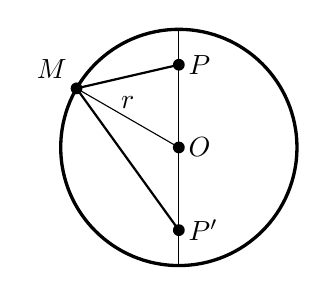
\begin{tikzpicture}[scale=1.5]
			          %projection ($(X)!(B')!(B)$)
			          %nommer chemin 'name path
			          %intersections \path [name intersections={of=d and gb,name=G}];
			          %intersection \path [name intersections={of=d and gb,by=G}];
			          %animation  \draw[visible on=<1>] 
				  %           \draw[visible on=<{2,4}>]
				  %angle arc[radius = 6mm, start angle= 180, end angle= 225] node [below left,pos=0.3]{$\alpha$}
				  %angle \pic [draw,"$\alpha$", angle eccentricity=1.5] {angle = A'--A--B};
				  %perpendiculaire ($(A')!3cm!-90:(A)$)
				  %cercle par point \node [draw] at (A) [circle through=(B)] {};
                                    \draw[very thick] (0,0) circle (1);
                                    \coordinate[label=right:$O$](O) at (0,0);
                                    \coordinate[label=right:$P$](P) at (0,0.7);
                                    \coordinate[label=right:$P'$](P') at (0,-0.7);
                                    \coordinate[label=above left:$M$](M) at (150:1);
                                    \draw[thick] (P) -- (M) -- (P');
                                    \fill (0,0) circle (0.05);
                                    \fill (P) circle (0.05);
                                    \fill (P') circle (0.05);
                                    \fill (M) circle (0.05);
                                    \draw (0,-1) -- (0,1);
                                    \draw (O)--  node[above ,pos=0.5] {$r$} (M);  
				  \end{tikzpicture}
				  \end{figure}
			
				  \begin{tcolorbox}[basic] 
				      
				    \smallskip
				    \hypotheses
							      
				    \these
				    \end{tcolorbox}
	
		
		\column{.5\textwidth}\centering
		
		\underline{Résolution}
		
                \begin{align*}
                  \vect{PM}\cdot\vect{P'M}=\ &(\vect{PO}+\vect{OM})\cdot(\vect{P'O}+\vect{OM}),\\[0.5em]
                  =\ & \vect{PO}\cdot\vect{P'O} + \vect{PO}\cdot\vect{OM} + \vect{OM}\cdot\vect{P'O}\\ &\hspace{20mm} + \vect{OM}\cdot\vect{OM},\\[0.5em]
                  =\ & \vect{PO}\cdot\vect{P'O} + \vect{OM}\cdot(\vect{PO}+\vect{P'O})\\ &\hspace{20mm} + \vect{OM}\cdot\vect{OM},\\[0.5em]
                  =\ & \vect{PO}\cdot\vect{P'O}+ \vect{OM}\cdot\vect{OM}, \textcolor{blue}{(2., 3.)}\\[0.5em]
                  =\ & (-\vect{OP})\cdot(-\vect{OP'})+ \vect{OM}\cdot\vect{OM},\\[0.5em]
                  =\ & (\vect{OP})\cdot(\vect{OP'})+ \vect{OM}\cdot\vect{OM},\\[0.5em]
                  =\ & |\vect{OP}||\vect{OP'}|\cos(180^\circ)\\ &\hspace{20mm} + |\vect{OM}||\vect{OM}|\cos(0),\\[0.3em]
                       =\ & -|\vect{OP}|^2 + r^2,\textcolor{blue}{( 3.)}\hspace{10mm} \qed
                  \end{align*}
		
		\heart
		
		%\centering\noindent\rule{2cm}{0.4pt}
              \end{columns}
               \notedir{%
	   .1 Prouver la thèse.
	   .2 Élément de théorie.
	   .3 Notions sur produit scalaire..
	   .2 Résolution.
	   .3 Décomposition de $PM$ et $PM'$ avec $O$..
           .4 Les constantes du problèmes sont $r$ et $|OP|$..
           .4 Produit scalaire distributif et commutatif..
           .3 $\vect{PO} = -\vect{PO'}$ vu hypothèses..
	   .3 Produit scalaire en termes de longueurs et angles..
           .3 Résultat est indépendant de la position de $M$..
           .3 Thèse vérifiée..
	   }
    }
	  
             \frame{ 
	  \enonce

	  \vfill\center
	  \underline{Résumé}\\ \flushleft
          \begin{itemize}
	  \item  Montrer qu’une expression vectorielle est constante =
            décomposer vecteurs pour éliminer le point variable.
          \item Trouver les constantes du problème pour savoir comment décomposer les vecteurs.
          \end{itemize}
    }
  
\end{document}

%%% Local Variables:
%%% mode: latex
%%% TeX-master: t
%%% End:
